% !TEX root = ./MParticle_resubmit.tex
\section{Standard Max Pressure Controller} \label{sec:immediatefeedback}
%This section summarizes results from \cite{MaxPressureStochastic} and \cite{MaxPressureOriginal} that we later extend.
%
%\subsection*{Principle}

Consider a weight assigned to each queue $(l,m)$ as a function of all network queue lengths $X$:
\begin{equation} \label{linkweight}
w(l,m)(X(t))= x(l,m)(t) - \sum_{p \in Out(m)} r(m,p)x(m,p)(t)
\end{equation}
where $Out(m)$ is the set of all links receiving flow from link $m$. 
%At time step $t+1$, the standard max pressure controller actuates the phase $S^* \in U$ which alleviates the most \emph{pressure} at the intersection based on feedback obtained at the immediately previous time step $t$. 
The \emph{pressure} $\gamma(S)$ that is potentially alleviated by a control action $S$ at time step $t$ is defined as follows: 
\begin{align}
\gamma(S)(X(t)) &= \sum_{l,m}c(l,m)w(l,m)(X(t))S(l,m)(t) \\
&= \sum_{l,m: S(l,m)(t) = 1}c(l,m)w(l,m)(X(t))
\end{align}
At each time step $t$, the standard max pressure controller $u^{*}(X(t))$ explicitly choses the phase $S^*\in U$ that maximizes $\gamma(S)(X(t))$:
\begin{equation} \label{original_MP}
%\boxed{ 
S^*(t)  = u^{*}(X(t)) = \arg\max\{\gamma(S)(X(t)) \vert S \in U\} 
%}
\end{equation}

Varaiya \cite{MaxPressureStochastic} shows the following stability result for the standard max pressure controller on a vertical queueing network:
\begin{Thm}\label{StabMP}
The max pressure control $u^{*}$ is stabilizing whenever the average demand vector $d = \lbrace d_{l}\rbrace$ is within the set of feasible demands $D^0$. There is no stabilizing control when $d\not \in D^0$.
\end{Thm}

%To prove this theorem, \cite{MaxPressureStochastic} shows that the quantity described in \eqref{stability_condition} is bounded when the controller is applied to the system dynamics \eqref{entrydynamics}-\eqref{internaldynamics}. It is however sufficient to show that there exists an $\varepsilon > 0$ such that
%\begin{equation} \label{stability_sufficient}
%\expectation{ \vert X(t+1)\vert_{2}^2 - \vert X(t)\vert_{2}^2  \big\vert X(t) } < -\varepsilon \vert X(t) \vert_{1} + K
%\end{equation}
%where $\vert X\vert_{2}^{2} = \sum_{l,m} \vert x(l,m)\vert^{2}$. This results from the fact that  \eqref{stability_sufficient}  implies:
%\begin{equation}
%\expectation{\vert X(T+1)\vert_{2}^2} - \expectation{\vert X(1)\vert_{2}^2} < -\varepsilon \sum_{t=1}^{T} \expectation{\vert X(t) \vert_{1}} + KT
%\end{equation}
%which can be rewritten as a bound on the desired quantity,
%\begin{equation} \label{IF_BOUNDS}
%\dfrac{\varepsilon}{T} \sum_{t=1}^{T} \expectation{\vert X(t) \vert_{1}}< K + \dfrac{1}{T}\expectation{\vert X(1)\vert_{2}^2}
%\end{equation}
%The detailed proof of Theorem \ref{StabMP} with an explicit definition of $\varepsilon$ and $K$, as originally derived in \cite{MaxPressureStochastic}, can be found in Appendix \ref{app_oldproof}. In the following sections we give three new original extensions of this proof corresponding to the following variations of max pressure control, illustrated in Figure \ref{fig:variations}:
%\begin{itemize}
%\item \emph{Cycle Max Pressure}: Queue states are observed at every time step, but the max pressure controller can only be applied every $\tau$ time steps. 
%\item \emph{Allocated Max Pressure}: Rather than a single optimal stage, the controller outputs  a convex combination of permissible stages to be applied at every time step.  
%\item \emph{Cycle-Allocated Max Pressure}: The controller applies a single convex combination of permissible stages for every $\tau$ time steps (a combination of the two above scenarios). 
%\end{itemize}
%\begin{figure}[h!]
%\centering
%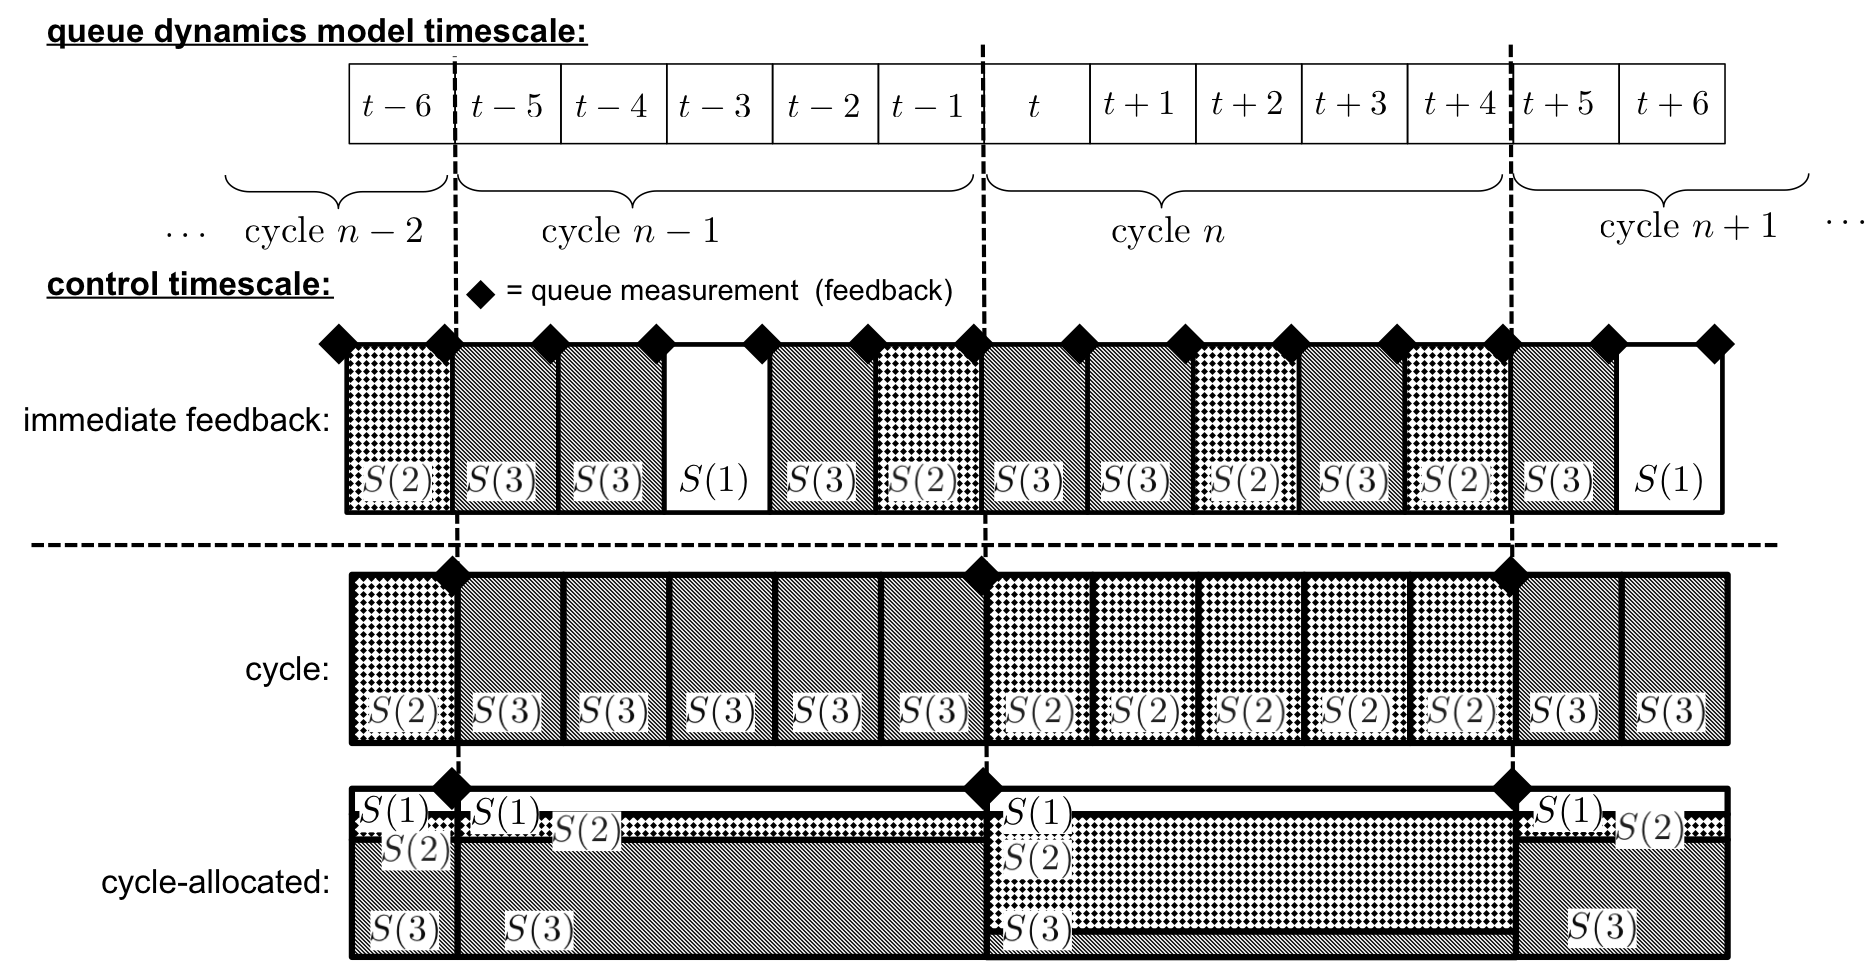
\includegraphics[width=\columnwidth]{./extensions_graphic.png}
%\caption{Extensions of max pressure modify the time scale of feedback and actuation. In this illustrations, consider three different feasible control actions represented by three degrees of shading. In the (original) immediate feedback formulation, measurements and control decisions are made at each model timestep; hence actuations can change as rapidly as queue states. \label{fig:variations}}
%\end{figure}
%
%

